\documentclass{article}
\voffset=-1.2cm
\oddsidemargin=0.0cm
\textwidth = 470pt
\usepackage{multicol}
\usepackage{amsmath}
\usepackage{framed}
\usepackage{amssymb}
\usepackage{graphicx}
\begin{document}
\tableofcontents
\newpage
\begin{framed}
\begin{verbatim}
4.1 What is a function?     
	 
4.1.1 Arrow diagram of a function   
4.1.2 Boolean functions and ordered n-tuples   
4.1.3 Absolute value function   
4.1.4 Floor and Ceiling Functions    
4.1.5 Polynomial functions    
4.1.6 Equality of functions  
\end{verbatim}
\end{framed}
\begin{framed}
\begin{verbatim}
4.2 Functions with Special Properties    

4.2.1 Encoding and decoding functions    
4.2.2 Onto functions     
4.2.3 One-to-one functions    
4.2.4 Inverse functions     
4.2.5 One-to-one correspondence   
\end{verbatim}
\end{framed}
\begin{framed}
	\begin{verbatim}
4.3 Exponential and Logarithmic functions   
 
4.3.1 Laws of exponents     
4.3.2 Logarithmic functions
\end{verbatim}
\end{framed}
\begin{framed}
	\begin{verbatim}
4.4 Comparing the size of functions    

4.4.1 O-notation     
4.4.2 Power functions    
4.4.3 Orders of polynomial functions    
4.4.4 Comparing the exponential and logarithmic functions with the power functions
4.4.5 Comparison of algorithms 
\end{verbatim}
\end{framed}

%======================================================================== %
\newpage
\section*{Arrow Diagrams for Functions}
\begin{itemize}
	\item Domain of a Function
	\item Co-Domain of a Function
	\item Range of a function
\end{itemize}

%--------------------------------------------%

\begin{itemize}
	\item one-one (surjective)
	\item onto (bijective)
\end{itemize}
%========================================================================= %
\newpage
\section*{Question Sheet}
Questions are taken from past papers of the ``Mathematics for Computing" syllabus.  They are re-arranged to correspond to the syllabus of this section.
%======================================================================== %


\newpage
\subsection*{Question 1 : 2010 part A}
\begin{figure}[h!]
	\centering
	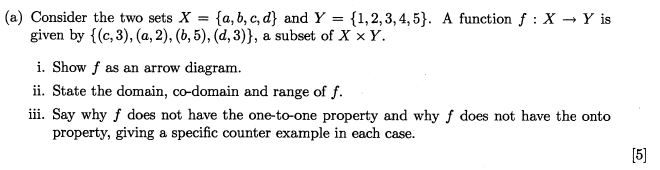
\includegraphics[width=1.1\linewidth]{FunctionsQuestion2010PartA}
	
\end{figure}
%======================================================================== %


\newpage
\subsection*{Question 2 : 2009 part A}
\begin{figure}[h!]
\centering
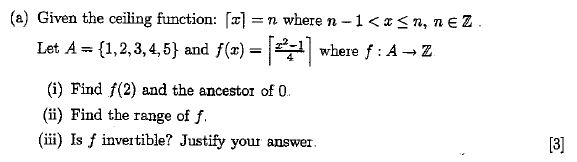
\includegraphics[width=1.01\linewidth]{FunctionsQuestion2009PartA}
\end{figure}
%======================================================================== %


\newpage
\subsection*{Question 3 : 2009 part B}
\begin{figure}[h!]
	\centering
	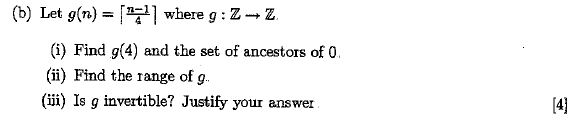
\includegraphics[width=1.21\linewidth]{FunctionsQuestion2009PartB}
	
\end{figure}
%======================================================================== %

\newpage
\subsection*{Question 4 : 2009 part B}
\begin{figure}[h!]
	\centering
	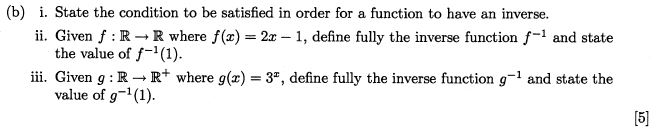
\includegraphics[width=1.1\linewidth]{FunctionsQuestion2010PartB}
	
\end{figure}
%======================================================================== %

\newpage
\subsection*{Question 5 : 2009 part B}

\begin{figure}[h!]
	\centering
	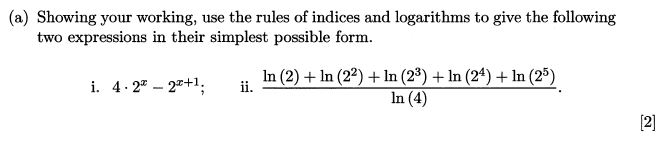
\includegraphics[width=1.1\linewidth]{FunctionsQuestion2012PartA}
	
\end{figure}

%======================================================================== %

\newpage
\subsection*{Question 6 : 2009 part B}
\begin{figure}[h!]
	\centering
	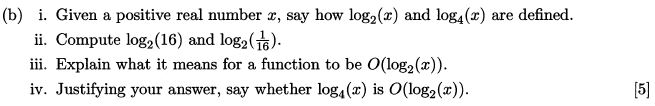
\includegraphics[width=1.1\linewidth]{FunctionsQuestion2012PartB}
	
\end{figure}

%======================================================================== %

\newpage
\subsection*{Question 7 : 2009 part B}
\begin{figure}[h!]
	\centering
	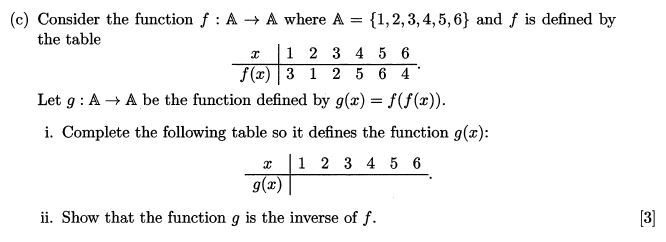
\includegraphics[width=1.1\linewidth]{FunctionsQuestion2012PartC}
	
\end{figure}

\newpage
%======================================================================== %


\newpage

\subsection*{Note: Invertible Functions}
A function is invertible if it fulfils two criteria
\begin{itemize}
	\item The function is \textbf{\textit{onto}},
	\item The function is \textbf{\textit{one-to-one}}.
\end{itemize}
\begin{framed}
State the conditions to be satisfied by a function
$f : X \leftarrow Y$ for it to have an inverse function
$f^{-1} : Y \leftarrow X$.
\end{framed}

%======================================================================== %
\section{Part 2}


\subsection*{Encoding and Decoding Functions (4.2)}


\subsection*{Onto Functions (4.2.2)}



%---------------------------------------------------------%

$\lceil \frac{x^2+1}{4} \rceil$
where $f : A \rightarrow \textbf{Z}$
\begin{itemize}
	\item[(i)] Find $f(4)$ and the ancestors of 3.
	\item[(ii)] Find the range of $f$.
	\item[(iii)] Is f invertible? Justify your answer
\end{itemize}

Given $f : \textbf{R} \rightarrow \textbf{R}$ where f(x) =3x-1,define fully
the inverse of the function f ,i.e.$f^{-1}$. 
State the value of $f^{-1}(2)$
%---------------------------------------------------------%

%======================================================================== %
\section{Part 3}
\subsection{Exponentials Functions}

\[ e^a \times e^b = e^{a+b}\]

\[ (e^a )^b = e^{ab}\]

%---------------------------------------------------------%
\subsection{Logarithmic Functions}

\subsubsection{Laws for Logarithms}
The following laws are very useful for working with logarithms.
\begin{enumerate}
	\item $\mbox{log}_b(X)$ + $\mbox{log}_b(Y)$ = $\mbox{log}_b(X\times Y)$
	\item $\mbox{log}_b(X)$ - $\mbox{log}_b(Y)$ = $\mbox{log}_b(X / Y)$
	\item $\mbox{log}_b(X^Y)$= $Y \mbox{log}_b(X)$
\end{enumerate}

\noindent \textbf{Question1.3} Compute the Logarithm of the following
\begin{itemize}
	\item $\mbox{log}_2(8)$
	\item $\mbox{log}_2(\sqrt{128})$
	\item $\mbox{log}_2(64)$
	\item $\mbox{log}_5(125)$ +   $\mbox{log}_3(729)$
	\item $\mbox{log}_2(64/4)$
\end{itemize}
%====================================== %




\section*{Question 4}

\subsection*{Part A : Functions}
Given a real number $x$, say how the floor of x  $\lfloor x \rfloor$ is defined.
\begin{itemize}
	\item[(i)] Find the values of $\lfloor 2.97 \rfloor$ and $\lfloor -2.97 \rfloor$.
	\item[(ii)] Find an example of a real number $x$ such that $\lfloor 2x \rfloor  \neq 2\lfloor x \rfloor$, justifying your answer.
\end{itemize}



%------------------------------------%
\subsection*{Part B : Logarithms}
Evaluate the following expression.
\[ \mbox{Log}_4 64 + \mbox{Log}_5 625 + \mbox{Log}_9 3 \] 


\subsection{Precision Functions}

\begin{itemize}
	\item Absolute Value Function $| x |$
	\item Ceiling Function $\lceil x \rceil$
	\item Floor Function  $\lfloor x \rfloor $
\end{itemize}
%\[ \lfloorx\rfloor\]

\noindent \textbf{Question1.2}: State the range and domain of the following function
\[ F(x) = \lfloor x-1 \rfloor \]
\subsection*{One-to-One Functions (4.2.3)}


\subsection*{One-to-One Functions (4.2.3)}
$f(x)$, must be \emph{One-to-One} and \emph{Onto}



\subsection*{Exponential and Logarithmic Functions (4.3)}

The Laws of Logarithms
\begin{itemize}
\item
\item $log_b(x^y) = y \times log_b(x)$
\item
\item
\end{itemize}

\subsection*{Comparing the size of Functions (4.4)}

Using O-notations

\subsection*{Power Notation (4.4.2)}


\subsection*{Section 8 Exercises}
\begin{itemize}
\item $8^{\frac{1}{3}}$ Recall $a^{\frac{b}{c}} = a^{\frac{b}{c}}$
\item
\item
\end{itemize}


\section{Mathematics for Computing: Onsite Tutorial two}

\textbf{Today's Class}
\begin{itemize}
\item Chapter 3: Logic
\begin{itemize}
\item
\item
\end{itemize}
\item Chapter 4: Functions
\begin{itemize}
\item Inverse of a Function
\item One-to-One and Onto
\item Special Functions
\end{itemize}
\end{itemize}
\newpage


\subsection*{The Asbolute Value, Floor and Ceiling Functions}
\begin{itemize}
\item The Absolute Value Function
\item Floor
\item Ceiling
\end{itemize}



\begin{itemize}
\item
\item
\item
\end{itemize}

\subsection*{Power functions and Polynomials}


Consider the function $f: Z \rightarrow Z$ defined by f(n) = 3n-1. Does this function have the onto property?
\[ax^2 + bx + c\]
%--------------------------------------------%
\subsection*{Summer 2003 Question 4}


\begin{center}
\begin{tabular}{ccccccc}
	x & & & & & & \\ \hline
	f(x) & & & & & & \\ \hline
	g(x) & & & & & & \\ \hline
\end{tabular}
\end{center}




\end{document}

